
%%%%%%%%%%%%%%%%%%%%%%%%%%%%%%%%%%%%%%%%%%%%%%%%%%%%%%%%%%%%%
\subsubsection{模型建立}

针对问题一，本节从关联分析和聚类分析两个角度建立模型。

\textbf{步骤1：Spearman秩相关模型}

对品类$a$和$b$的日销售量序列$S_{a,t}$和$S_{b,t}$，将其转换为秩次$R(S_{a,t})$和$R(S_{b,t})$，计算Spearman秩相关系数：
\begin{equation}
  \rho_{ab} = \frac{\text{Cov}(R(S_a), R(S_b))}{\sigma(R(S_a)) \cdot \sigma(R(S_b))} = 1 - \frac{6\sum_t d_t^2}{n(n^2-1)}
\end{equation}
其中$d_t = R(S_{a,t}) - R(S_{b,t})$，$n=1049$为观测天数。$\rho_{ab}>0$表示两品类销售量呈同向变动趋势，$\rho_{ab}<0$表示反向变动。

\textbf{步骤2：K-means++聚类模型}

对159个销售天数$\geq 30$的单品，构建特征向量$\mathbf{x}_j = (\bar{s}_j, \sigma(s_j), \text{CV}(s_j), \bar{p}_j)$，经对数变换后进行K-means++聚类。目标函数为簇内平方和最小化：
\begin{equation}
  \min_{C_1,\ldots,C_K} \sum_{k=1}^{K} \sum_{\mathbf{x} \in C_k} \|\mathbf{x} - \boldsymbol{\mu}_k\|^2
\end{equation}
其中$\boldsymbol{\mu}_k$为簇$k$的质心。最优$K$通过轮廓系数最大化选择：
\begin{equation}
  \text{Sil}(K) = \frac{1}{N}\sum_{j=1}^{N} \frac{b(j) - a(j)}{\max\{a(j), b(j)\}}
\end{equation}
其中$a(j)$为样本$j$到同簇其他样本的平均距离，$b(j)$为到最近异簇的平均距离。

\textbf{步骤3：分布拟合}

对每个品类的日销售量序列，分别拟合正态、对数正态和Gamma分布，通过Kolmogorov-Smirnov检验的$p$值选择最优分布。

\subsubsection{模型求解}

基于上述模型，本节利用Python（scipy.stats, scikit-learn）进行求解。K-means++聚类采用加权概率初始化策略\cite{Arthur2007}，$K$值在2--7范围内搜索，以轮廓系数最大化为选择准则——$K=2$时Silhouette$=0.463$，$K=3$时降至$0.398$，$K=4$时$0.356$，$K$继续增大轮廓系数单调下降，且簇规模严重失衡（最小簇仅6个单品），因此确定$K=2$。随机种子42，重启动次数10，10次重启标签一致率100\%。

求解得到以下结果。Spearman秩相关系数矩阵如图\ref{fig:spearman}所示，$\rho$范围为$[-0.194, 0.625]$，均值$|\rho|=0.395$。花叶类与花菜类的正相关最强（$\rho=0.625$），花叶类与食用菌次之（$\rho=0.590$）。茄类与水生根茎类呈唯一负相关（$\rho=-0.194$），茄类与其他品类的关联普遍较弱（$|\rho|<0.33$）。

\begin{figure}[H]
  \centering
  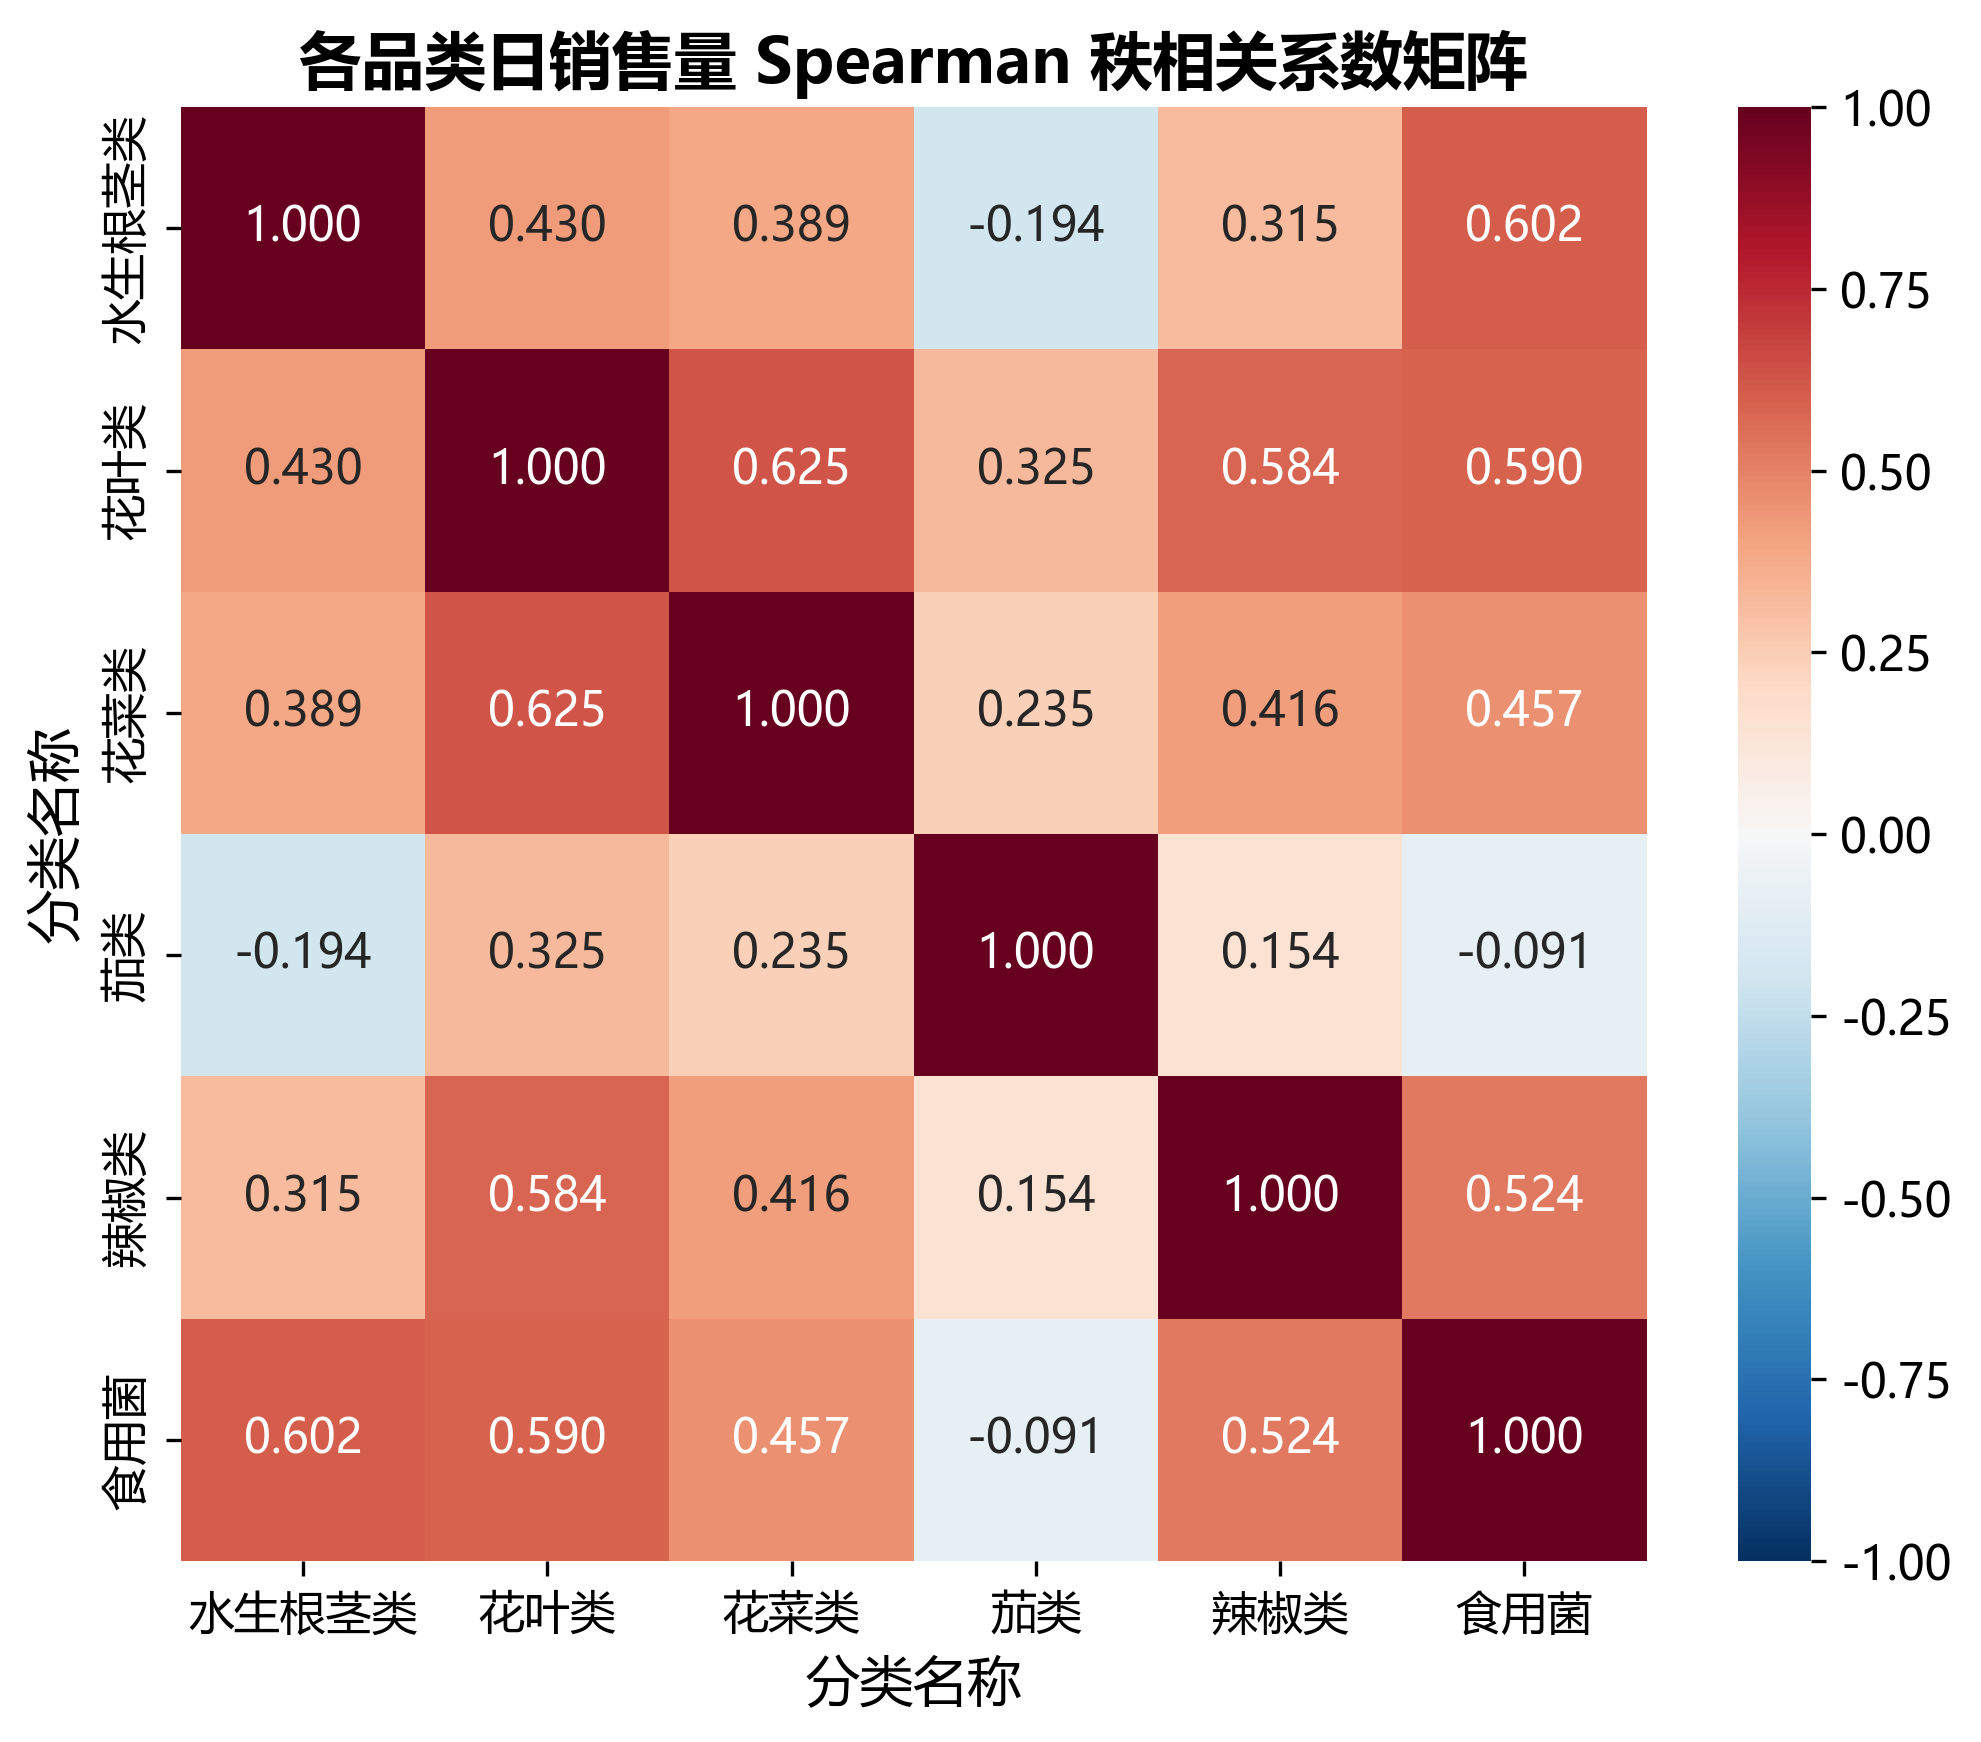
\includegraphics[width=0.85\textwidth]{figures/fig1_spearman_corr.png}
  \caption{各品类日销售量Spearman秩相关系数矩阵}
  \label{fig:spearman}
\end{figure}

Bootstrap重抽样（100次）表明相关估计稳定，平均$\rho$标准差$0.026$。跨年分析显示2020--2021年$\rho$向量高度一致（$r=0.824$），2021--2022年相关性减弱（$r=0.168$），主要源于茄类品类的持续萎缩（日均销量从26 kg降至19 kg，仅10个单品导致估计不稳定）和疫情后消费模式调整。

K-means++聚类在$K=2$时轮廓系数最大（$0.463$），$K=3$时降至$0.398$。轮廓系数$0.463$处于中等偏弱水平，原因可能有二：蔬菜单品销售模式本身呈连续谱分布而非离散簇；特征向量仅含销量统计量，未纳入品类、季节等结构化信息。尽管轮廓系数不高，$K=2$的划分仍具有业务可解释性（低量高波动vs高量中波动），且跨随机种子稳定（10次重启标签一致率100\%）。作为对比，层次聚类（Ward联结）在$K=2$时轮廓系数为$0.412$，略低于K-means++，支持当前选择。簇0（72个单品）以辣椒类和食用菌为主，特征为低销量（均值$2.2$ kg/天）、高波动（$\text{CV}=0.76$）、高价格（$12.96$元/kg）；簇1（87个单品）以花叶类为主，特征为高销量（均值$12.4$ kg/天）、中等波动（$\text{CV}=0.83$）、低价格（$6.18$元/kg）。两簇内均包含全部六个品类，表明品类内部也存在销量分化。

分布拟合结果表明，对数正态分布是蔬菜日销售量最适用的分布族，花叶类（KS $p=0.544$）、花菜类（$p=0.879$）和茄类（$p=0.991$）均不拒绝对数正态假设。

月度销售量趋势如图\ref{fig:monthly}所示，花叶类在11月达到峰值，花菜类和食用菌在秋冬季节销售旺盛，呈现出明显的季节性模式。

\begin{figure}[H]
  \centering
  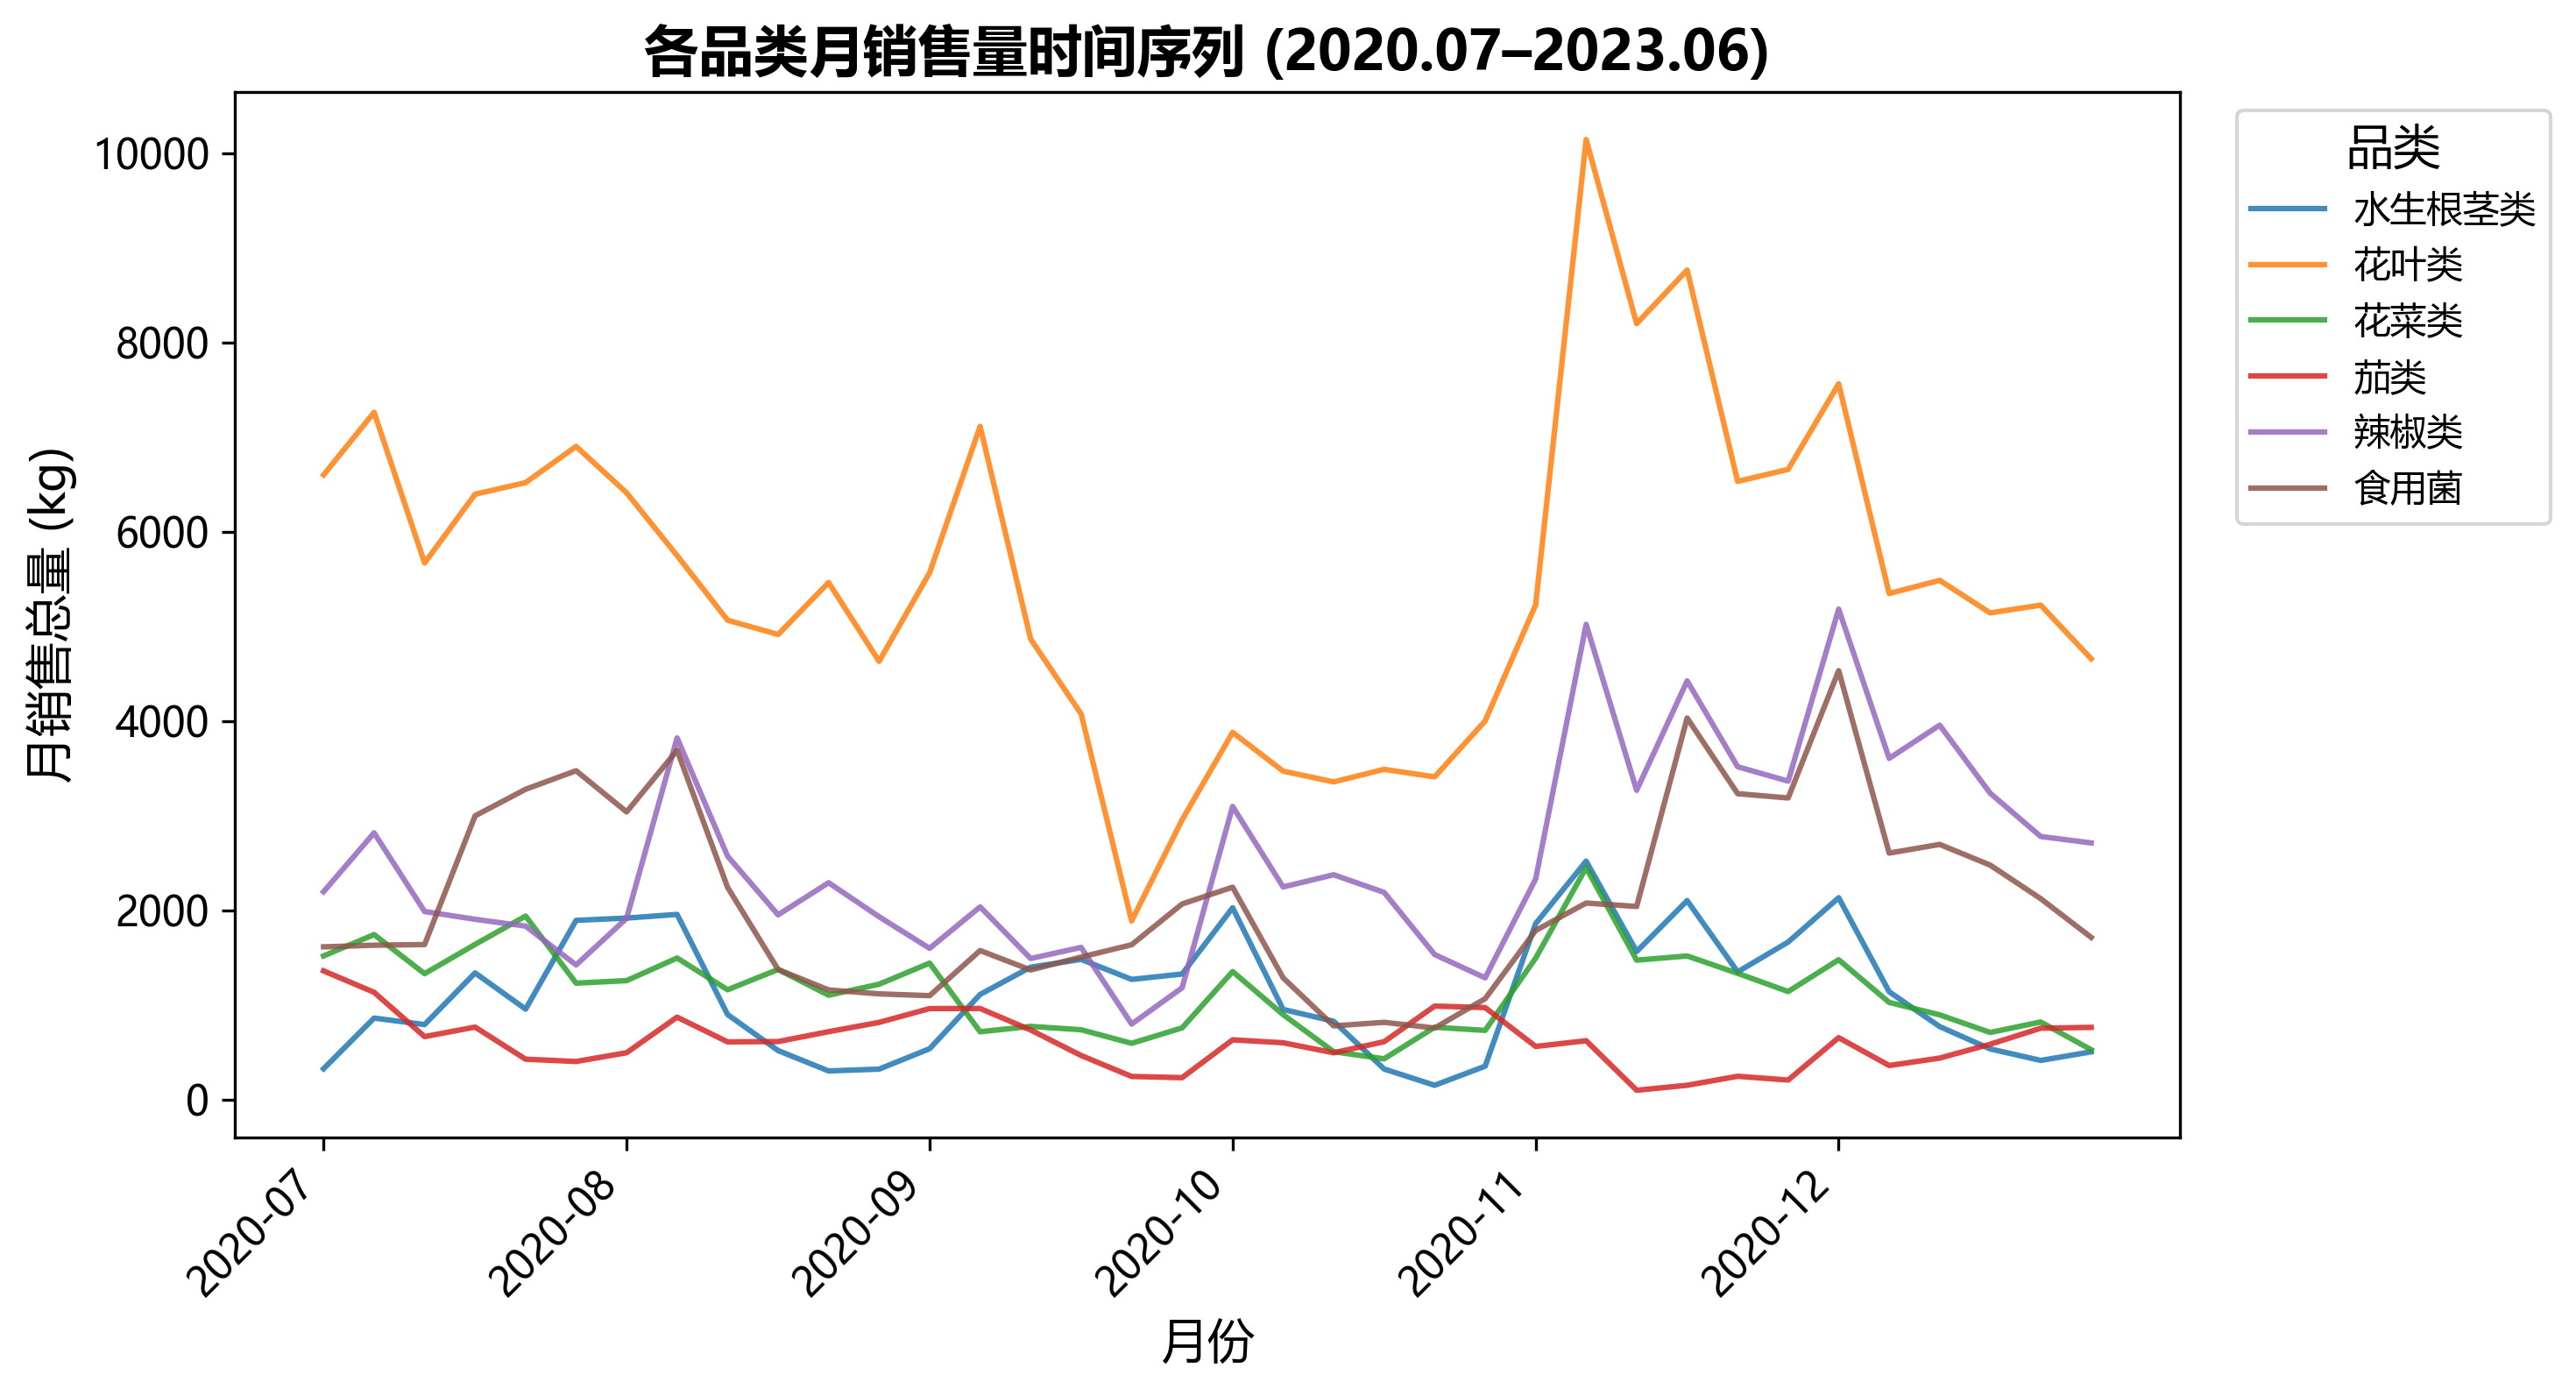
\includegraphics[width=0.95\textwidth]{figures/fig2_monthly_trend.png}
  \caption{各品类月销售量时间序列（2020.07--2023.06）}
  \label{fig:monthly}
\end{figure}

以上分析表明，六个品类间存在差异化的Spearman关联结构：花叶类--花菜类--食用菌高度协同（ρ>0.5），茄类相对独立（|ρ|<0.33）。单品按销量规模和波动性聚为低量高波动和高量中波动两类，对数正态分布是蔬菜日销售量最适用的分布族。这些结论分别用于问题二的品类需求特征选择和问题三的单品多样性约束设计。
